\documentclass{esg8012pset}
\begin{preamble}
  \usepackage{amsmath}
  \usepackage{amssymb}
  \usepackage{enumerate}
  \usepackage{graphicx}
  \usepackage{hyperref}
  %\usepackage{siunitx}
  \providecommand{\uvec}[1]{{\hat{\bf{#1}}}}
  \usepackage{pgf,tikz}
  \usetikzlibrary{arrows}
  \makeatletter
  \newcommand{\interitemtext}[1]{%
    \begin{list}{}
     {\itemindent=0mm\labelsep=0mm
     \labelwidth=0mm\leftmargin=0mm
     \addtolength{\leftmargin}{-\@totalleftmargin}}
      \item #1
    \end{list}
  }
  \makeatother
  \renewcommand{\d}{\,d}
  \providecommand{\norm}[1]{\lVert#1\rVert}
\end{preamble}

\classname{Physics 8.012}
\semester{Fall 2010}
\problemsetnumber{8}
\makeatletter
\duedate{Friday, November 12}
\readingassignment{Kleppner and Kolenkow, \emph{An Introduction to Mechanics}, Chapter Six}

\begin{document}

\noindent Problems: Chapter 6: 1, 2, 4, 6, 7, 10, 13


\begin{problem}{K\&K 6.1}
  \begin{enumerate}[(a)]
    \item Show that if the total linear momentum of a system of particles is zero, the angular momentum of the system is the same about all origins. Explain how you may apply this result involving an elastic collision of two rigid bodies.
    \item Show that if the total force on a system of particles is zero, the torque on the system is the same about all origins. Explain how you can use this result for static equilibrium problems.
  \end{enumerate}
\end{problem}
\begin{solution}
  \begin{enumerate}[(a)]
    \item Let $I$ be the (possibly (uncountably) infinite) index set of particles.  Assume that $\displaystyle \sum_{\alpha\in I} m_\alpha \vec v_\alpha = 0$.  Then $\vec L_{s\alpha} = \vec r_{s\alpha} \times m_\alpha \vec v_\alpha$, so $$\displaystyle \vec L_{s} = \sum_{\alpha\in I}\vec r_{s\alpha} \times m_\alpha \vec v_\alpha.$$  Similarly, $$\displaystyle \vec L_{s'} = \sum_{\alpha\in I}\vec r_{s'\alpha} \times m_\alpha \vec v_\alpha.$$  But then \begin{align*}
    \vec L_{s'} & = \sum_{\alpha\in I}(\vec r_{s\alpha} + \vec r_{s's}) \times m_\alpha \vec v_\alpha \\
    & = \sum_{\alpha\in I}\vec r_{s\alpha} \times m_\alpha \vec v_\alpha + \vec r_{s's} \times \sum_{\alpha\in I} m_\alpha \vec v_\alpha \\
    & = \vec L_{s'} + \vec r_{s's} \times \sum_{\alpha\in I} m_\alpha \vec v_\alpha \\
    & = \vec L_{s'}
    \end{align*} \par
    This may be applied in the center of mass reference frame to the collision.  FIX (Explain how you may apply this result involving an elastic collision of two rigid bodies.)
    \item Let $I$ be the (possibly (uncountably) infinite) index set of particles.  Assume that $\displaystyle \sum_{\alpha\in I} \vec F_\alpha = 0$.  Then $\vec \tau_{s\alpha} = \vec r_{s\alpha} \times \vec F_\alpha$, so $$\displaystyle \vec \tau_{s} = \sum_{\alpha\in I}\vec r_{s\alpha} \times \vec F_\alpha.$$  Similarly, $$\displaystyle \vec \tau_{s'} = \sum_{\alpha\in I}\vec r_{s'\alpha} \times \vec F_\alpha.$$  But then \begin{align*}
    \vec \tau_{s'} & = \sum_{\alpha\in I}(\vec r_{s\alpha} + \vec r_{s's}) \times \vec F_\alpha \\
    & = \sum_{\alpha\in I}\vec r_{s\alpha} \times \vec F_\alpha + \vec r_{s's} \times \sum_{\alpha\in I} \vec F_\alpha \\
    & = \vec \tau_{s'} + \vec r_{s's} \times \sum_{\alpha\in I} \vec F_\alpha \\
    & = \vec \tau_{s'}
    \end{align*} \par
    This may be applied in the center of mass reference frame. FIX (Explain how you can use this result for static equilibrium problems.)
  \end{enumerate}
\end{solution}




\begin{problem}{K\&K 6.2}
  A drum of mass $m_A$ and radius $a$ rotates freely with initial angular velocity $\omega_{A,0}$. A second drum with mass $m_B$ and radius $b > a$ is mounted on the same axle and is at rest, although it is free to rotate. A thin layer of sand with mass $m_S$ is distributed on the inner surface of the smaller drum. At $t = 0$, small perforations in the inner drum are opened. The sand starts to fly out at a constant rate $\lambda$ and sticks to the outer drum. Find the subsequent angular velocities of the two drums $\omega_A$ and $\omega_B$. Ignore the transit time of the sand.
  \begin{center}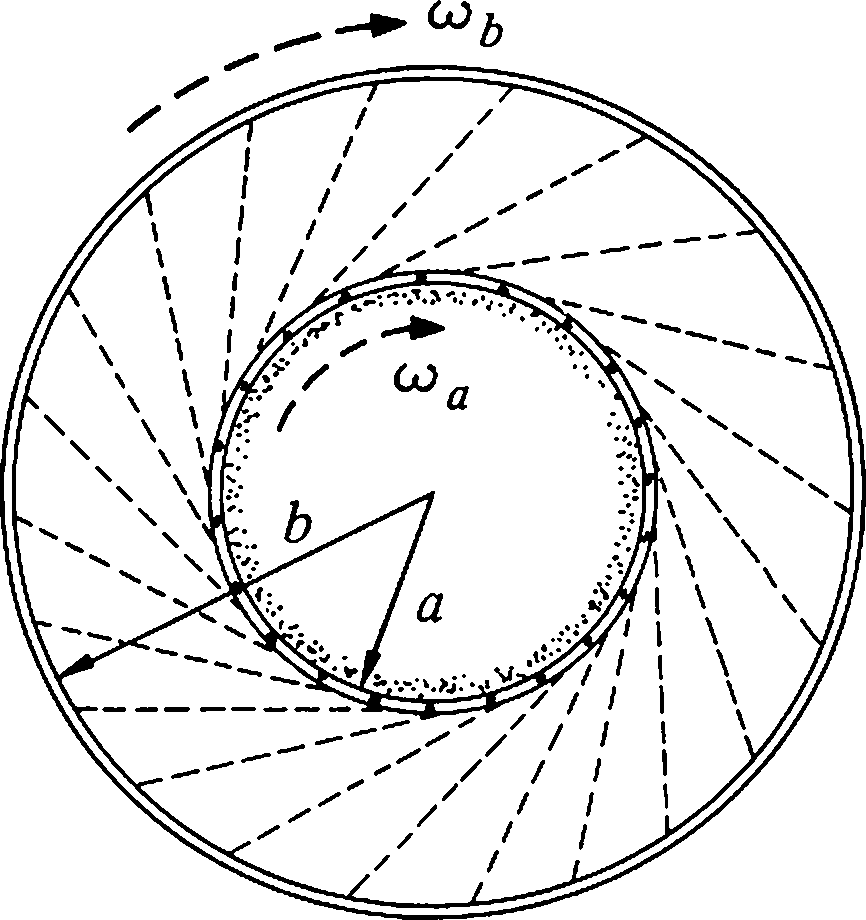
\includegraphics[width=0.2\textwidth]{ps08_1}\end{center}
\end{problem}
\begin{solution}
  \begin{center}
  \definecolor{qqwuqq}{rgb}{0,0.39,0}
  \begin{tikzpicture}[line cap=round,line join=round,>=triangle 45,x=1.0cm,y=1.0cm]
  \clip(-4,-4) rectangle (4,4);
  \draw [shift={(2.34,2.72)},color=qqwuqq,fill=qqwuqq,fill opacity=0.1] (0,0) -- (-130.71:0.6) arc (-130.71:-90:0.6) -- cycle;
  \draw(0,0) circle (2.34cm);
  \draw(0,0) circle (3.59cm);
  \draw (0,0)-- (2.34,2.72);
  \draw (0,0)-- (2.34,0);
  \draw [dash pattern=on 4pt off 4pt] (2.34,0)-- (2.34,2.72);
  \draw [domain=-4:4] plot(\x,{(--12.87-2.34*\x)/2.72});
  \draw[color=black] (1.46,1.3) node {$b$};
  \draw[color=black] (1.22,-0.18) node {$a$};
  \draw[color=qqwuqq] (2.44,2.44) node {$\theta$};
  \end{tikzpicture}
  \end{center}
  The sand, when leaving the inner drum, has linear velocity $\omega_{A,t}a$.  The component of the velocity which is tangent to the outer drum is $\omega_{A,t}a\sin\theta = \omega_{A,t}\frac{a^2}{b}$.  Then, for sand of mass $\d m$, since (angular) momentum is conserved, $\d m \omega_{A,t}\frac{a^2}{b} + m_B \omega_{B,t} b = (m_B + \d m)\omega_{B,t+\d t}b$, or $\d m \omega_{A,t}\frac{a^2}{b^2} + m_B \omega_{B,t} = (m_B + \d m)\omega_{B,t+\d t}$.  Then \begin{align*}
  \Delta m \omega_{A,t}\frac{a^2}{b^2} + m_B \omega_{B,t} & = (m_B + \Delta m)(\omega_{B,t} + \Delta \omega_{B, t}) \\
  \Delta m \omega_{A,t}\frac{a^2}{b^2} + m_B \omega_{B,t} & = m_B \omega_{B,t} + m_B \Delta \omega_{B, t} + \Delta m \omega_{B,t} + \Delta m \Delta \omega_{B, t} \\
  \Delta m \omega_{A,t}\frac{a^2}{b^2} & = m_B \Delta \omega_{B, t} + \Delta m \omega_{B,t} + \Delta m \Delta \omega_{B, t} \\
  \frac{\d m}{\d t} \omega_{A,t}\frac{a^2}{b^2} & = m_B \frac{\d \omega_{B, t}}{\d t} + \frac{\d m}{\d t} \omega_{B,t} \\
  \frac{\d m}{m_{B, t}} & = \frac{\d \omega_{B, t}}{\omega_{A,t}\frac{a^2}{b^2} - \omega_{B,t}} \\
  \intertext{Since $\omega_{A, t}$ is constant,}
  \int_{m = m_B}^{m_B + \lambda t}\frac{\d m}{m_{B, t}} & = \int_{\omega_{B, t} = \omega_{B, 0}}^{\omega_{B, t}}\frac{\d \omega_{B, t}}{\omega_A\frac{a^2}{b^2} - \omega_{B,t}} \\
  \ln\frac{m_B + \lambda t}{m_B} & = \ln\frac{\omega_A\frac{a^2}{b^2} - \omega_{B,0}}{\omega_A\frac{a^2}{b^2} - \omega_{B,t}} \\
  \frac{m_B + \lambda t}{m_B} & = \frac{\omega_A\frac{a^2}{b^2} - \omega_{B,0}}{\omega_A\frac{a^2}{b^2} - \omega_{B,t}} \\
  \omega_A\frac{a^2}{b^2} - \omega_{B,t} & = m_B\frac{\omega_A\frac{a^2}{b^2} - \omega_{B,0}}{m_B + \lambda t} \\
  \omega_{B,t} & = \omega_A\frac{a^2}{b^2} - \frac{m_B}{m_B + \lambda t}\left(\omega_A\frac{a^2}{b^2} - \omega_{B,0}\right) \\
    & = \omega_A\frac{a^2}{b^2}\left(1 - \frac{m_B}{m_B + \lambda t}\right) + \omega_{B,0}\frac{m_B}{m_B + \lambda t} \\
    & = \omega_A\frac{a^2}{b^2}\cdot \frac{\lambda t}{m_B + \lambda t} + \omega_{B,0}\frac{m_B}{m_B + \lambda t}
  \end{align*}
\end{solution}




\begin{problem}{K\&K 6.4}
  A spaceship is sent to investigate a planet of mass $m_p$ and radius $r_p$. While hanging motionless in space at a distance $5 r_p$ from the center of the planet, the ship fires an instrument package with speed $v_0$. The package has mass $m_i$ which is much smaller than the mass of the spacecraft. The package is launched at an angle $\theta$ with respect to a radial line between the center of the planet and the spacecraft. For what angle $\theta$ will the package just graze the surface of the planet.
  \begin{center}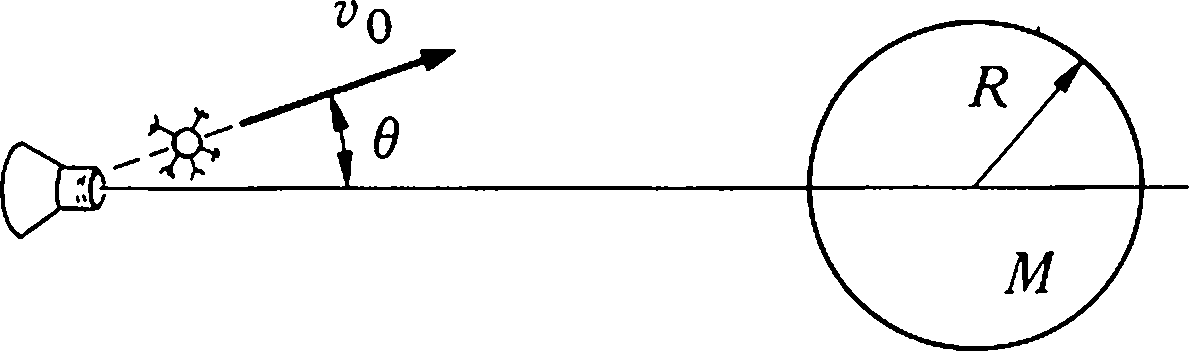
\includegraphics[width=0.4\textwidth]{ps08_2}\end{center}
\end{problem}
\begin{solution}
  Assume that $m_p \gg m_i$.  Since there are no external forces, mechanical energy is constant.  Since there are no external torques and the forces are along the line between the planet and the instrument package, the angular momentum about the center of the planet is constant.  If it just glances the planet, then the velocity is perpendicular to the radius, and the distance is $r_p$.  Then
  \begin{align*}
    E_0 = K_0 + U_0 & = \frac{1}{2}m_i v_0^2 - G\frac{m_i m_p}{5 r_p} \\
    E_f = K_f + U_f & = \frac{1}{2}m_i v_f^2 - G\frac{m_i m_p}{r_p} \\
    \\
    \frac{1}{2}m_i v_0^2 - G\frac{m_i m_p}{5 r_p} & = \frac{1}{2}m_i v_f^2 - G\frac{m_i m_p}{r_p} \\
    \frac{1}{2}m_i \left(v_0^2 - v_f^2\right) & = G \frac{m_i m_p}{r_p} \left(\frac{1}{5} - 1\right) \\
    \frac{1}{2}m_i \left(v_f^2 - v_0^2\right) & = G \frac{4 m_i m_p}{5 r_p} \\
    v_f^2 - v_0^2 & = G \frac{8 m_p}{5 r_p} \\
    v_f^2 & = G \frac{8 m_p}{5 r_p} + v_0^2 \\
    \\
    \\
    \vec L_0 & = \vec r_0 \times m_i \vec v_0 \\
    & = 5 r_p m_i v_0\sin\theta \\
    \vec L_f & = \vec r_f \times m_i \vec v_f \\
    & = r_p m_i \sqrt{G \frac{8 m_p}{5 r_p} + v_0^2} \\
    \\
    5 r_p m_i v_0\sin\theta & = r_p m_i \sqrt{G \frac{8 m_p}{5 r_p} + v_0^2} \\
    5 v_0\sin\theta & = \sqrt{G \frac{8 m_p}{5 r_p} + v_0^2} \\
    \sin\theta & = \frac{1}{5}\sqrt{G \frac{8 m_p}{5 r_p v_0^2} + 1}
  \end{align*}


  %\definecolor{qqwuqq}{rgb}{0,0.39,0}
  %\begin{tikzpicture}[line cap=round,line join=round,>=triangle 45,x=1.0cm,y=1.0cm]
  %\clip(-1,-2) rectangle (9,2);
  %\draw [shift={(0,0)},color=qqwuqq,fill=qqwuqq,fill opacity=0.1] (0,0) -- (0:0.6) arc (0:32.88:0.6) -- cycle;
  %\draw [shift={(6.62,0)},color=qqwuqq,fill=qqwuqq,fill opacity=0.1] (0,0) -- (167.98:0.6) arc (167.98:180:0.6) -- cycle;
  %\draw(6.62,0) circle (1.46cm);
  %\draw [->,line width=1.6pt] (0,0) -- (1.64,1.06);
  %\draw (6.62,0)-- (1.64,1.06);
  %\draw (0,0)-- (6.62,0);
  %\draw[color=qqwuqq] (1,0.24) node {$\theta$};
  %\draw[color=qqwuqq] (5.98,0.16) node {$\theta'$};
  %\draw[color=black] (1.14,1.18) node {$v_0$};
  %\end{tikzpicture}
  %\begin{align*}
  % \vec x_0 & = \vec 0 \\
  % \vec v_0 & = v_0\cos\theta_0\hat i + v_0\sin\theta_0\hat j \\
  % m_i \vec {\ddot x} & = -G\frac{m_i m_p}{\vec x \cdot \vec x}\hat r \\
  % m_i \vec{\ddot x} & = -G\frac{m_i m_p}{\vec x \cdot \vec x}\cdot \frac{\vec x - (5 r_p \hat i)}{(\vec x - (5 r_p \hat i))\cdot(\vec x - (5 r_p \hat i))}  \\
  %  %& = -G\frac{m_i m_p}{\vec x \cdot \vec x}\cdot \frac{\vec x - 5 r_p \hat i}{\vec x \cdot \vec x - 10 r_p \hat i \cdot \vec x  - (5 r_p \hat i))\cdot(\vec x - (5 r_p \hat i))} \\
  %\end{align*} FIX
  %
  %
\end{solution}


\begin{problem}{K\&K 6.6}
  A person of mass $m$ is standing on a railroad car which is rounding an unbanked turn of radius $R$ at a speed $v$. His center of mass is at a height of $L$ above the car midway between his feet which are separated by a distance of $d$. The man is facing the direction of motion. What is the magnitude of the normal forces on each foot?
  \begin{center}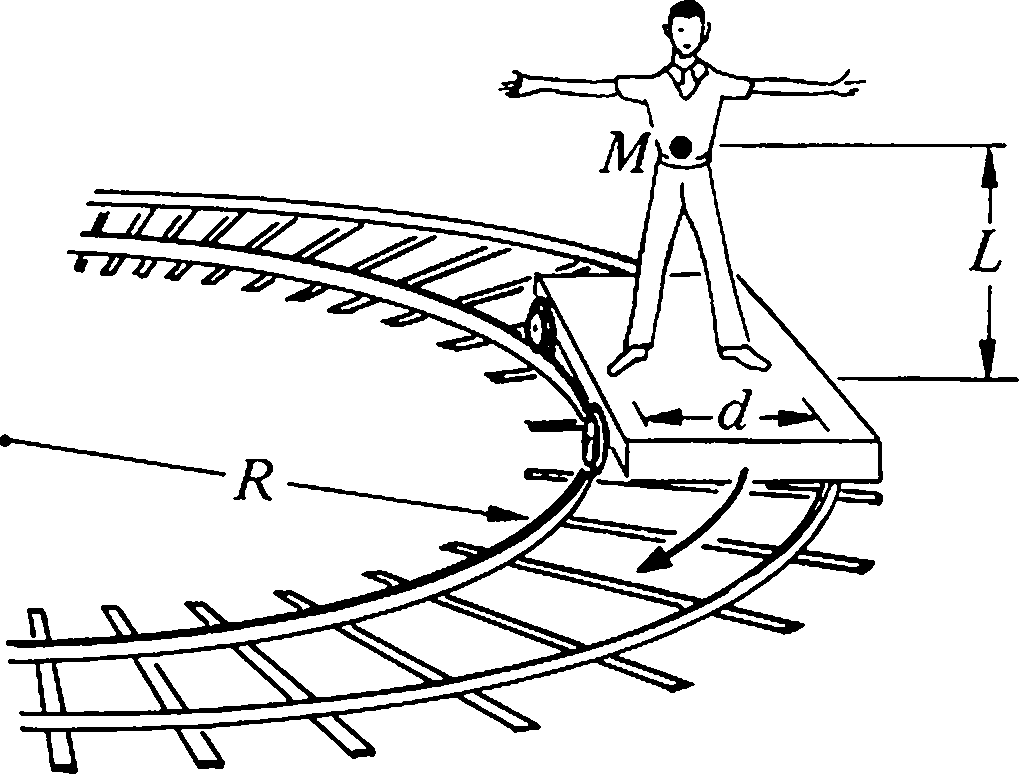
\includegraphics[width=0.4\textwidth]{ps08_3}\end{center}
\end{problem}
\begin{solution}
  The centripetal force on the person is $\frac{m v^2}{R + \frac{d}{2}}$.  If $F_1$ and $F_2$ are the forces of friction on the inward and outward foot, respectively, then $$F_1 + F_2 = \frac{m v^2}{R + \frac{d}{2}}$$ and $$m g = N_1 + N_2.$$  Let $\theta$ denote the angle from the vertical to a leg.  Then $\tan\theta = \frac{d}{2L}$.  Finally, since the person is not rotating about the center of mass, $(N_1 - N_2)\sqrt{\frac{d^2}{4} + L^2}\sin\theta + (F_1 + F_2)\sqrt{\frac{d^2}{4} + L^2}\cos\theta = 0$, so $((N_1 - N_2)\sin\theta + (F_1 + F_2)\cos\theta)\sqrt{\frac{d^2}{4} + L^2} = 0$, so $(N_1 - N_2)\tan\theta + (F_1 + F_2) = 0$.  Plugging in $\tan\theta$, $$(N_1 - N_2)\frac{d}{2L} + (F_1 + F_2) = 0.$$  Then \begin{align*}
  0 & = (N_1 - N_2)\frac{d}{2L} + \frac{m v^2}{R + \frac{d}{2}} \\
  N_2 - N_1 & = \frac{m 2L v^2}{d R + \frac{d^2}{2}} \\
    & = \frac{4 m L v^2}{2 d R + d^2} \\
  N_2 + N_1 & = m g \\
  \\
  2N_2 & = mg + \frac{4 m L v^2}{2 d R + d^2} \\
  2N_1 & = m g - \frac{4 m L v^2}{2 d R + d^2} \\
  \\
  N_1 & = \frac{m g}{2} - \frac{2 m L v^2}{2 d R + d^2} \\
  N_2 & = \frac{m g}{2} + \frac{2 m L v^2}{2 d R + d^2}
  \end{align*}
\end{solution}




\begin{problem}{K\&K 6.7}
  \begin{enumerate}[(a)]
    \item Find the moment of inertia of a thin sheet of metal of mass $m$ in the shape of an isosceles right triangle about an axis that passes through one vertex of the sheet, perpendicular to the plane of the sheet. The length of the two equal sides is $s$.
    \item Find the moment of inertia of a thin sheet of metal of mass $m$ in the shape of an isosceles right triangle about an axis that passes through the same vertex of the sheet, but aligned along one side of length $s$ (in the plane of the sheet).
  \end{enumerate}
\end{problem}
\begin{solution}
  \begin{enumerate}[(a)]
    \item Suppose the triangle is rotating with angular velocity $\omega$.  Then \begin{align*}
      \vec L & = \lim_{\Delta m\to 0} \sum_{i} \vec r_i \times \Delta m_i \vec v_i \\
      & = \lim_{\Delta m\to 0} \sum_{i} \vec r_i \times \Delta m_i (\vec \omega \times \vec r_i) \\
      & = \lim_{\Delta m\to 0} \sum_{i} \vec r_i \times \Delta m_i (\vec \omega \times \vec r_i) \\
    \intertext{Since all of these vectors are perpendicular,}
      & = \lim_{\Delta m\to 0} \sum_{i} r_i \Delta m_i (\omega r_i) \\
      & = \omega \lim_{\Delta m\to 0} \sum_{i} r_i^2 \Delta m_i \\
      & = \omega \int \d m r^2 \\
      & = \omega \iint_0^s (x^2 + y^2)\d m \\
      & = \omega m \iint_0^s (x^2 + y^2)\d y\d x \\
      & = \omega m \int_0^s \int_0^{s-x} (x^2 + y^2)\d y\d x \\
      & = \omega m \int_0^s \left.\left(y x^2 + \frac{y^3}{3}\right)\right|_0^{s-x} \d x \\
      & = \omega m \int_0^s \left((s-x)x^2 + \frac{(s-x)^3}{3}\right) \d x \\
      & = \omega m \int_0^s \left(sx^2 - x^3 + \frac{(s-x)^3}{3}\right) \d x \\
      & = \omega m \left( \int_0^s sx^2 - x^3 \d x - \int_s^0 \frac{(s-x)^3}{3} \d (s-x) \right) \\
      & = \omega m \left( \left.\frac{sx^3}{3} - \frac{x^4}{4}\right|_0^s - \left.\frac{(s-x)^4}{12}\right|_{s-x=s}^0 \right) \\
      & = \omega m \left( \frac{s^4}{3} - \frac{s^4}{4} + \frac{s^4}{12}\right) \\
      & = \omega m \left( \frac{s^4}{12} + \frac{s^4}{12}\right) \\
      & = \omega m \frac{s^4}{6} \\
    I & = m \frac{s^4}{6}
    \end{align*}
    \item Suppose the triangle is rotating with angular velocity $\omega$.  Then \begin{align*}
      \vec L & = \lim_{\Delta m\to 0} \sum_{i} \vec {r_i}_{\bot} \times \Delta m_i \vec v_i \\
      & = \lim_{\Delta m\to 0} \sum_{i} \vec {r_i}_{\bot} \times \Delta m_i (\vec \omega \times \vec r_i) \\
      & = \lim_{\Delta m\to 0} \sum_{i} \vec {r_i}_{\bot} \times \Delta m_i (\vec \omega \times \vec {r_i}_{\bot}) \\
    \intertext{Since all of these vectors are perpendicular,}
      & = \lim_{\Delta m\to 0} \sum_{i} {r_i}_{\bot} \Delta m_i (\omega {r_i}_{\bot}) \\
      & = \omega \lim_{\Delta m\to 0} \sum_{i} {{r_i}_{\bot}}^2 \Delta m_i \\
      & = \omega \int \d m {{r_i}_{\bot}}^2 \\
      & = \omega m \iint (x^2)\d y \d x \\
      & = \omega m \int_0^s (x^2)(s-x) \d x \\
      & = \omega m \left(s\int_0^s (x^2) \d x - \int_0^s x^3 \d x\right) \\
      & = \omega m \left(\frac{s^3}{3} - \frac{s^4}{4}\right) \\
      & = \omega m s^3 \cdot \frac{4-3s}{12} \\
    I & = m s^3 \cdot \frac{4-3s}{12}
    \end{align*}
  \end{enumerate}
\end{solution}



\begin{problem}{K\&K 6.10}
  A cylinder of mass $m$ and radius $R$ is rotated in a V groove with constant angular velocity $\omega_{0}$.
The coefficient of friction between the cylinder and the surface is $\mu$. What external torque must be applied to the cylinder to keep it rolling?
  \begin{center}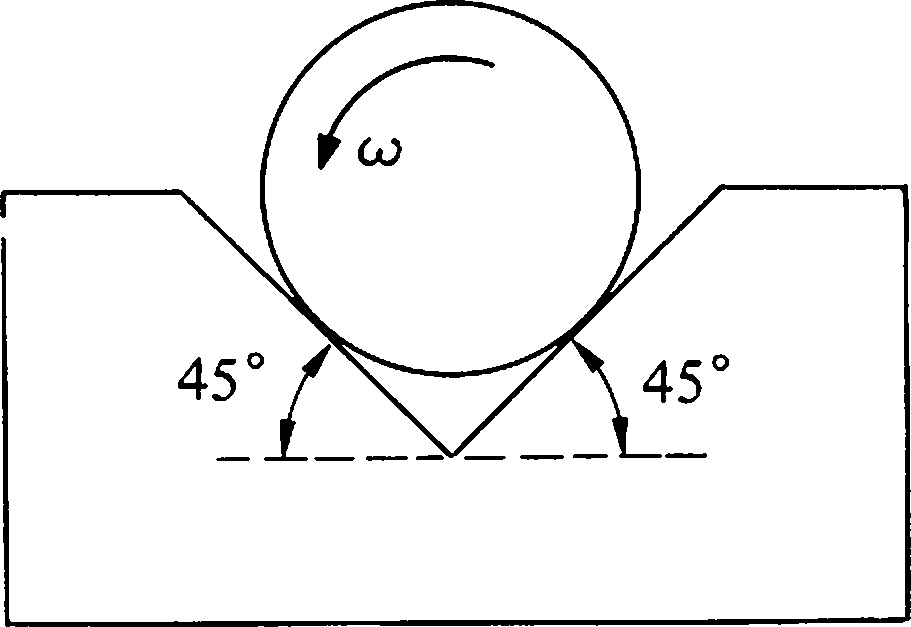
\includegraphics[width=0.3\textwidth]{ps08_4}\end{center}
\end{problem}
\begin{solution}
  \newcommand{\degre}{\ensuremath{^\circ}}
  \definecolor{uququq}{rgb}{0.25,0.25,0.25}
  \definecolor{zzttqq}{rgb}{0.6,0.2,0}
  \definecolor{qqwuqq}{rgb}{0,0.39,0}
  \begin{tikzpicture}[line cap=round,line join=round,>=triangle 45,x=1.0cm,y=1.0cm]
  \clip(-5.1,-2.1) rectangle (5.1,6);
  \draw [shift={(0,0)},color=qqwuqq,fill=qqwuqq,fill opacity=0.1] (0,0) -- (0:0.6) arc (0:45:0.6) -- cycle;
  \draw [shift={(0,0)},color=qqwuqq,fill=qqwuqq,fill opacity=0.1] (0,0) -- (135:0.6) arc (135:180:0.6) -- cycle;
  \fill[color=zzttqq,fill=zzttqq,fill opacity=0.1] (5,3.2) -- (3.2,3.2) -- (0,0) -- (-3.2,3.2) -- (-5,3.2) -- (-5,-2) -- (5,-2) -- cycle;
  \draw [color=zzttqq] (5,3.2)-- (3.2,3.2);
  \draw [color=zzttqq] (3.2,3.2)-- (0,0);
  \draw [color=zzttqq] (0,0)-- (-3.2,3.2);
  \draw [color=zzttqq] (-3.2,3.2)-- (-5,3.2);
  \draw [color=zzttqq] (-5,3.2)-- (-5,-2);
  \draw [color=zzttqq] (-5,-2)-- (5,-2);
  \draw [color=zzttqq] (5,-2)-- (5,3.2);
  \draw [dash pattern=on 3pt off 3pt] (3.2,0)-- (-3.2,0);
  \draw(0,3.3) circle (2.33cm);
  \draw [->,line width=1.6pt] (1.65,1.65) -- (1.65,-0.04);
  \draw [->,line width=1.6pt] (1.65,1.65) -- (0.81,2.5);
  \draw [->,line width=1.6pt] (1.65,1.65) -- (0.89,0.89);
  \draw[color=qqwuqq] (0.8,0.36) node {$45\textrm{\degre}$};
  \draw[color=qqwuqq] (-0.86,0.3) node {$45\textrm{\degre}$};
  \fill [color=uququq] (1.65,1.65) circle (1.5pt);
  \draw[color=black] (1.92,0.98) node {$F_g$};
  \draw[color=black] (1.24,2.7) node {$F_n$};
  \draw[color=black] (1.36,0.88) node {$F_{fr}$};
  \end{tikzpicture}

  The normal force is $F_N = F_g \cos 45^{\circ} = \frac{m g}{\sqrt{2}}$.  Then the total frictional force is $\sqrt{2}\mu m g$, so the torque must be $R m g \sqrt{2} \mu$.
\end{solution}




\begin{problem}{K\&K 6.13}
  A body of particle of mass $m$ (treat it as a point like particle) is attached to a post of radius $R$ by a string. Initially it is a distance $r_0$ from the center of the post and it is moving tangentially with a speed $v_0$. In case (a) the string passes through a hole in the center of the post at the top. The string is gradually shortened by drawing it through the hole. In case (b) the string wraps around the outside of the post. What quantities remain constant in each case? Find the final speed of the body when it hits the post for each case.
  \begin{center}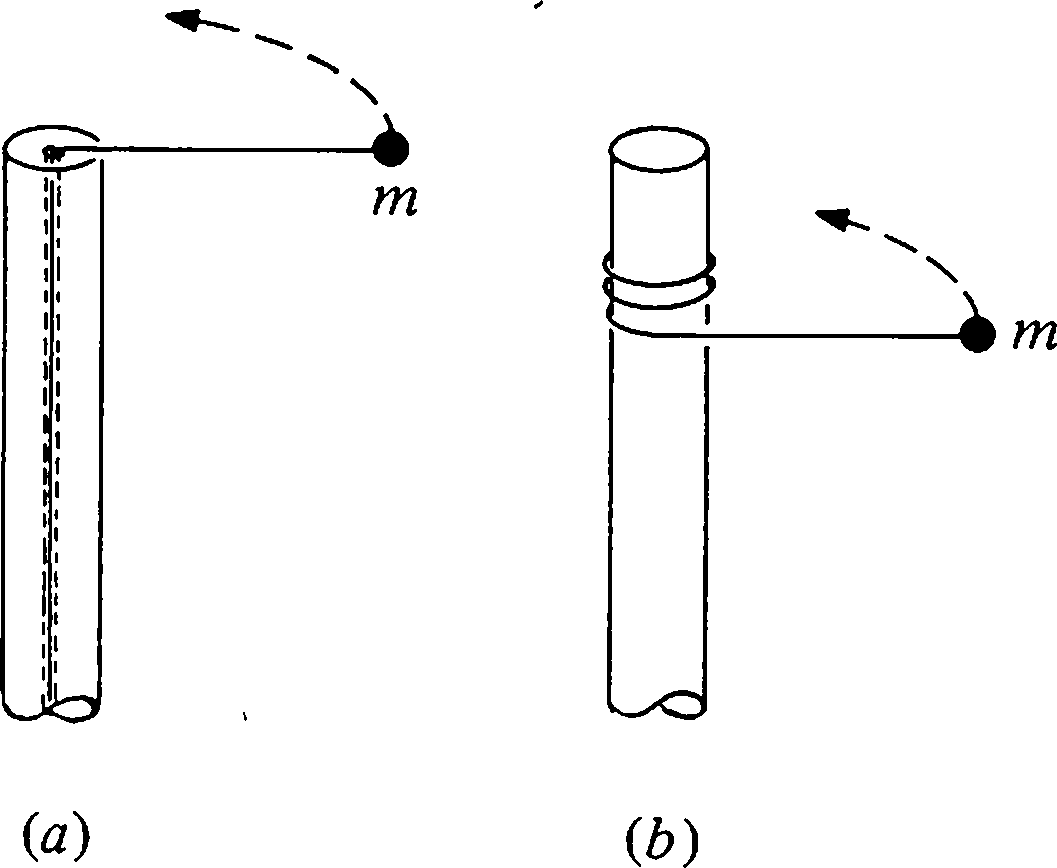
\includegraphics[width=0.3\textwidth]{ps08_5}\end{center}
\end{problem}
\begin{solution}
  \begin{enumerate}[(a)]
    \item Angular momentum remains constant because the force is only in the radial direction.  Then \begin{align*}
      \vec L_0 & = \vec r_0 \times m \vec v_0 \\
      \vec L_f & = \vec R \times m\vec v_f \\
      \intertext{Since the velocity is perpendicular to the radius,}
      r_0 m v_0 & = R m v_f \\
      v_f & = \frac{r v_0}{R}
    \end{align*}
    \item Mechanical energy remains constant because there are no external forces.  Since we neglect potential energy, speed remains constant.
  \end{enumerate}
\end{solution}

\end{document}
